% using Elseveir template per https://www.elsevier.com/authors/author-schemas/latex-instructions
% model paper: Dynamic effects of teacher turnover on the quality of instruction (2016)
%   Hanushek et al
%   from Economics of Education Review

% secondary model paper: The effects of economic policy and political uncertainties on economic activities
% Gholipour, 2019
% https://www.sciencedirect.com/science/article/pii/S0275531918306081
\documentclass[review]{elsarticle}

\usepackage{lineno,hyperref}
\modulolinenumbers[5]

\journal{Journal of \LaTeX\ Templates}
\bibliographystyle{elsarticle-num}
\usepackage{booktabs}
\usepackage{graphicx}
\graphicspath{{../alt-ed-survey/figures-and-tables}}
\usepackage{hyperref}
\usepackage{threeparttable}  
\usepackage{tikz}
\usetikzlibrary{calc,matrix}

% ref: https://tex.stackexchange.com/questions/19390/how-do-you-download-packages-for-texworks-on-windows-7
% ref: https://tex.stackexchange.com/questions/47418/siunitx-specifying-custom-command-as-input-symbol
\newcommand{\sym}[1]{\rlap{#1}}
\usepackage{siunitx}
\sisetup{ detect-mode, 
          group-digits            = false ,
          input-signs             = ,
          input-symbols           = ()[]-+* , % specifying \sym here does not work
          input-open-uncertainty  = ,
          input-close-uncertainty = ,
          table-align-text-post   = false 
        }

\usepackage{tabularx}

\begin{document}
\begin{frontmatter}

\title{
    Dynamic Effects of H-1B and Section 127 Policy Interaction on Higher Education
    \tnoteref{titlenotes}
}
% \tnotetext[titlenotes]{
%     Go to \url{https://github.com/Vandivier/research-dissertation-case-for-alt-ed/tree/master/papers/}
%     for additional materials including the online appendix,
%     survey data, and data analysis source code.
% }

\author[mymainaddress]{John Vandivier} % \fnref{authorlinefootnote}}
\address[mymainaddress]{4400 University Dr, Fairfax, VA 22030}
\ead{jvandivi@masonlive.gmu.edu}

\begin{abstract}
    % role model abstract based on Hanushek et al (2016)
    % model length = 151 words
    % this abstract length = 165 words
    % narrative-problem-solution structure
    % ---
    It is widely believed that employer educational assistance increases the quantity demanded for higher education,
    but the original passage of Section 127 which enables this tax-deduction for employers is associated with a reduction to the growth of higher education enrollment,
    and a simple regression of the assistance limit on total enrollment indicates a significant negative correlation. % technically, `reg totalen emp' in my data set
    This raises concerns that confounding factors bias estimates of the effectiveness of Section 127 assistance.
    After taking extensive steps to account for policy effects and other dynamic economic factors,
    I robustly identify a positive effect on enrollment from employer educational assistance
    by exploiting real variation in employer educational assistance over the 27-year period from 1990 to 2016.
    Results are validating using panel vector autoregression (PVAR),
    dynamic least squares (DOLS) methods,
    and instrumental variable (IV) approaches.
    In the preferred model,
    an increase in tax-deductable employer educational assistance
    in the amount of one dollar is associated with
    an increase of about 600 to national total enrollment in institutions of higher education.

    % Highlights
    % 1. Section 127 Employer Assistance
    % 2. 
    % 3. 
    % 4. 

    % % alternate role model abstract based on Gholipour
    % % model length = 129 words
    % % this abstract length = 91 words
    % % technical micropaper structure
    % % ---
    % This paper explores the dynamic effects of Section 127, veteran education benefits, Stafford loan, and H-1 Visa policy
    % on total enrollment in the United States
    % using annual data from degree-granting institutions in the United States during the 27-year period from 1990 to 2016.
    % By applying panel vector autoregression (PVAR) and dynamic least squares (DOLS) methods,
    % the results show that a positive shock to Section 127 assistance triggers a positive response from enrollment in the short-run.
    % In addition, I find that higher levels of assistance do not significantly decrease enrollment in the long-run.
\end{abstract}

\begin{keyword}
education economics, section 127, educational assistance, veteran education, h-1b, debt crisis, dols, vars
\MSC[2010] % TODO
\end{keyword}
\end{frontmatter}

\pagebreak
\linenumbers

    \section{Introduction}

    % TODO: basic descriptive time series line graphs.
    % enrollment, loans, prices, and policy states over time are candidates.

    % background scratch notes in this comment block:
    % degree requirement as a strategy to import cheap, effective foreign labor (VISA)
    % this prevents high school graduates from directly entering roles that typically award section 127 (white color, major employer, corporate work)
    % until recently, that is, with walmart, mcdonalds, starbucks giving section 127 i think even to part timers
    % Theory: After 1990, companies began requiring a 4 year degree so they could have an H-1B justification.
    % This caused more americans to pursue an undergraduate degree without section 127. we should see section 127 use decline after 1990.
    % Revisit in conclusion -> Recently, employers have begun giving the benefit anyway due to labor selection and internal ROI benefits

    Basic supply and demand theory indicate that a reduction in price is associated with an increase to the quantity demanded.
    In 1978, a bill was passed allowing employer educational assistance to be tax-deductable in the United States up to a nominal limit of 5,000 dollars.
    It is surprising, therefore, that 1978 is associated with a local decrease in the growth rate on both total and public university enrollment.
    This study exploits real variation in the tax-deductable employer educational assistance limit to eventually identify the expected positive effect,
    but not before identifying and correcting for several interesting things going on in the economy.
    Specifically, an interaction between H-1B policy and Section 127 employer educational assistance is discovered and assessed.

    \subsection{Supply-Side Explanations}
    Before forming more exotic theories, some simpler hypotheses should be checked.
    One hypothesis is that there is an adjustment period after the passage of Section 127 and before widespread employer provision of the newly deductable benefit.
    Allowing for a 3 or 5 year lag around the passage of Section 127 in 1978 does not resolve the issue.
    Across the eight five-year periods from 1970 to 2010, the five-year public enrollment growth rate was above 9 percent as often as it was below.
    Two of the four low-rate intervals occured immediately subsequent to the 1978 creation of Section 127.
    The interval just prior, from 1970-1975, saw the highest growth in enrollment across the period.
    It does not appear to be a one-year fluke that the employer educational assistance is associated with declined enrollment growth.
    
    Another important point is that Section 127 was passed in 1978, but it took effect in the 1979 tax year.
    1979 saw modest growth in enrollment,
    but given the pre-existing long-run context of positive trend in enrollment,
    it is not clear that Section 127 can be attributed any causality.

    An alternative to the 3 or 5 year lagged analysis is to directly refer to surveys of employers.
    Cappelli\cite{cappelli2004employers} identifies 3 employer surveys from 1992 and 1993 which indicate that at least 86 percent of surveyed employers provided educational assistance.
    These studies were samples of convenience with a focus on large employers,
    but additional information leads Cappelli to claim that a substantial majority of employers offer such plans over his period of analysis from about 1990 to 2004.
    Cappelli notes that employee utilization of the benefit favors graduate education
    with about 20 percent of graduate students receiving employer assistance
    and roughly 6 percent of undergraduates doing so.
    Common provision of the benefit has remained true in later years.
    In 2013, SHRM reported that 61 percent of employers offer tuition assistance\cite{cherry2014rejuvenating}.
    In 2017, World at Work found that 85 percent of employers offered such a benefit,
    with another 7 percent offering non-reimbursement tuition assistance, such as upfront tuition discounts\cite{talentculture_2018}.

    \subsection{H-1B, Veteran Education Benefits, and Stafford Loan Interaction}
    The idea that graduate students mainly use employer education benefits motivates hypotheses around undergraduate access.
    Increasingly since the 1990s, developed economies have experienced degree inflation and experience inflation.
    Entry level positions now require a degree when previously this was not necessary, even when technology has made the work easier.
    It is possible that undergraduate access to employer benefits are reduced simply because employers increasingly hire individuals that already have the degree.
    Employers are known to value the degree as a signal of labor quality, but these days there are plenty of other, richer data sources on quality for certain professions.
    In computer programming we see some employers completely dropping the degree requirement and preferring technical interviews, digital portfolio evaluation, and other signals.
    Why, then, do other leading employers continue to require the degree?
    One answer is that the degree requirement forms an H-1B justification.
    Since the passage of the Immigration Act of 1990\cite{law1990law}, a corporation must claim a shortage of qualified specialized labor to justify an H-1B.
    The "attainment of a bachelor's or higher degree" is written into the law as a test of whether labor is qualified and specialized.
    This would motivate employers to begin requiring the degree in order to obtain cheap immigrant labor, even while knowing the degree may not be necessary.

    Zero employers offered Section 127 educational assistance in 1977, but the majority offered the benefit by 1993.
    Immigration policy is a change which interrupts this period of analysis, but there are two other major policies to take note of.
    Stafford loans were available before Section 127, but the limits and rules for these loans and other government assistance to higher education fluctuated over the period of analysis.
    Government educational benefits for veterans is another major policy in the higher education assistance space.
    It becomes difficult to imagine a proper Section 127 analysis which does not include dynamic correction for these potentially important factors,
    as well as correction for general price changes and economic conditions in the economy over time.
    Such a corrected analysis is exactly what this paper completes.

    \subsection{Demand-Side Explanations}
    The prior explanations consistitute a supply-side exploration of the impotence of Section 127.
    An alternative explanation is that there simply wasn't much demand for college in the early years of Section 127.
    Indeed, lack of market demand appears to be a good explanation for the consistent college-age enrollment percent
    which is observed at 25.7 percent in both 1970 and 1980.
    A demand-side explanation is consistent with the falling average tuition and fees observed for all institutions from 1972 to 1980.
    After 1980 we see an upward trend in price and also an upward trend in college-age enrollment percentage, as well as simple total enrollment.

    With an increase to the Stafford limit in the 1977 school year,
    a major change to veteran education benefits in the 1981 school year,
    Section 127 beginning in the 1978 school year,
    and price changes in higher education and for all other goods,
    claims about a particular cause become dubious without full and corrective statistical treatment.
    Even so,
    there is some plausibility to the claim that Section 127 was passed during a time when demand was weak,
    so that there may have been a positive effect on the part of Section 127 as early as the first year,
    but it was overshadowed by general decline.
    The main contribution of this line of thought to a more general analysis is that corrective statistics should include price data
    for education in particular, and also for the general economy.

    \section{Empirical Model}

    Equation \ref{eq1} is an ordinary least squares model of total enrollment higher education in the United States.

    \begin{equation}
        Y = \beta_1X_1+\beta_2X_2...+\beta_kX_k+e
        \label{eq1}
    \end{equation}

    The Section 127 policy effect is the variable of interest.
    Three other policy variables are included for federal lending policy, veteran education benefits, and H-1 Visa policy.
    In addition to the four policy variables, 
    enrollment is modelled as a function of time,
    and the price of tuition and fees.
    A variable for personal consumption expenditures (PCE) as an measure of inflation is also included.

    For robustness and analytical completeness, I test two other left hand variables using ordinary least squares,
    then I also test the relation of interest with two other modelling approaches.
    Specifically, I explore vector autoregressive (VAR) models
    and an instrumental variable regression following the Anderson–Hsiao pattern\cite{anderson1981estimation} with the lagged variable of interest as an instrument.

    \section{Data}

    Information on total enrollment for all degree-granting postsecondary institutions in the United States
    is provided by the National Center for Education Statistics (NCES)\cite{nces_2019}.
    Enrollment figures are for the fall semester of the school year.
    Information on selected years from 1947 to 2028 is provided, where values for 2018 and later are projected.
    The present study does not use any of the projected values.
    Other data sources and policy considerations constrain the period of interest to the 27-year period from 1990 to 2016.    
    % total enrollment: https://nces.ed.gov/programs/digest/d18/tables/dt18_303.10.asp

    Personal Consumption Expenditures (PCE) data is a measure of inflation provided by the U.S. Bureau of Economic Analysis (BEA)\cite{bea_2020}.
    Education-specific inflation is also calculated using NCES data\cite{nces_2017}.
    NCES data is the average tuition and required fees for full-time undergraduate students across all degree-granting postsecondary institutions.
    NCES provides nominal values and values adjusted for the consumer price index (CPI) for tuition.
    The price of room and board is ignored.
    % https://fred.stlouisfed.org/series/PCE
    % https://nces.ed.gov/programs/digest/d17/tables/dt17_330.10.asp

    Nominal Section 127 limits are a matter of public law.
    Section 127 took effect beginning after December 31, 1978 with a nominal assistance limit of 5,000 dollars\cite{plaw95_600_1978}.
    In October 1986, Pub. L. 99–514 increased the nominal assistance limit to 5,250 dollars\cite{plaw99_514_1986}.
    Real Section 127 employer assistance limits are calculated two ways.
    One variable is constructed for each measure of inflation.
    Price deflators for each measure of inflation use 2016 as a base year.
    
    % begin discuss veteran benefits data
    Changes to veteran education benefits are also a matter of public law.
    A categorical variable is used to capture the state of veteran education benefits among five possible states over the period from 1970 to 2020.
    The Servicemen's Readjustment Act of 1944,
    also called the G.I. Bill,
    is the first interesting case of veteran benefits,
    but it precedes the period of interest for this study.

    The original bill expired in 1956\cite{glass_2010}.
    This expired state is the first state represented by the veteran education state variable.
    The Veterans Educational Assistance Program (VEAP) was established in 1981\cite{veteransaffairs_2017}.
    A third period of interest begins in 1984 with the enactment of the Montgomery GI Bill\cite{powers_2018}.
    A fourth period of interest begins in 2009 with the Post-9/11 GI Bill.

    Finally, many benefits from the Forever GI Bill became effective in 2018,
    with additional provisions taking effect in 2020 and 2022\cite{veteransaffairs_2020}.
    This fifth policy state is too recent to be included in the period of interest.
    The recent changes in veteran education benefits are a critical caveat for any attempt at forecasting or prediction outside of the period of study.

    Due to constraints on the availability of other right hand variable data,
    the main period of regression analysis ranges from 1990 to 2016.
    Veteran education benefits exhibit only one change during this period,
    but this factor proves to be significant in the preferred model.
    % GI Bill accounting https://en.wikipedia.org/wiki/G.I._Bill#Chapter_30_(Montgomery_GI_Bill)
    % Variable implemented as categorical
    % [state A] original bill was 1944-1984
    % [state B] VEAP established 1981 https://www.benefits.va.gov/gibill/veap.asp
    % [state C] Montgomery GI went into effect 1984
    % [state D] Post-9/11 GI Bill went into effect for 2009 school year https://www.thebalancecareers.com/gi-bill-for-the-21st-century-3347143
    % [state E] Forever GI bill rolls out new benefits starting in 2018 https://rebootcamp.militarytimes.com/education-transition/education/2017/08/16/trump-signed-the-forever-gi-bill-here-are-11-things-you-should-know/
    %
    % end discuss veteran benefits data

    Stafford loan data is another key component of the analysis.
    Stafford loan data is directly relevant by itself,
    but it is further intended a proxy for broader non-military federal student aid policy.
    There are two variables for Stafford loans.
    The first is the nominal loan limit for undergraduates.
    The second is a dummy variable indicating whether the undergraduate loan limit
    is the combined limit for undergraduate and graduate loans.
    A policy change became effective in 1993 which grouped these limits together.
    Stafford loan data is sourced from FinAid\cite{finaid_2020}.
    % TODO: should I dive into an explanation for focus on undergraduate education? not doing for now.

    Visa policy is a complex issue.
    Annual H-1B visa award is an important and simple variable used for the purposes of this study.
    The Immigration Act of 1990 decomposed the existing H-1 visa into distinct H-1A and H-1B categories.
    Over time, H-1B1 and H-1C classifications were established,
    and many other important but less relevant classifications outside of the H-1 family exist as well.
    The H-1B visa is most relevant for this study because it specifically relates to the undergraduate degree.
    The Immigration Act of 1990 makes available the H-1B classification for specialized workers,
    or workers in a specialty occupation.
    A specialty occupation is formally defined as "an occupation that requires...attainment of a bachelor's or higher degree..."

    H-1 visas are a subgroup of nonimmigrant visas.
    Nonimmigrant visa award data by classification from 1987 to 2019 is provided by
    the Bureau of Consular Affairs within the United States State Department\cite{bureauof_2020}.
    This paper exclusively uses the most relevant H-1B visa award numbers,
    but reanalysis with other visa classifications could yield statistically significant findings.
    The prior H-1 visa was also a merit worker visa, but it had no formal definition of merit.
    In 1989, 48,820 H-1 visas were awarded.
    In 1991, 7,443 H-1A visas were awarded, and 51,882 H-1B visas were awarded.
    It's plausible that the college-educated effect informally existed prior to the 1990 legislation.
    One might also find small but significant effects by looking into visas outside the H-1 family.
    Besides the number of actual visa awards, an analyst could look for visa cap effects,
    or visa policy state effects.
    For example, Pew Research Center notes that the American Competitiveness in the 21st Century Act of 2000 exempts certain entities from the H-1B cap\cite{ruiz2017key}.
    % ref: https://en.wikipedia.org/wiki/H-1B_visa#H-1B_visas_issued_per_year
    % more state variable food https://redbus2us.com/h1b-visa-total-cap-history-from-1990-to-current-year/
    % 1952 allows unlimited merit immigration, 1990 there is a quota and degree requirement added to H-1B: https://en.wikipedia.org/wiki/H-1B_visa#Immigration_Act_of_1990
    % A crackdown in 2017: https://www.investopedia.com/news/impact-trumps-h1b-visa-crackdown-5-charts/
    % other policies for policy state analysis:
    %   https://en.wikipedia.org/wiki/Legal_Immigration_Family_Equity_Act#V_visa
    %   not sure it's relevant - https://en.wikipedia.org/wiki/Immigration_Reform_and_Control_Act_of_1986
    %   https://en.wikipedia.org/wiki/H-1B_Visa_Reform_Act_of_2004
    %   1986 we get h-2a and h-2b https://www.uscis.gov/ilink/docView/AFM/HTML/AFM/0-0-0-1/0-0-0-13593/0-0-0-13614.html
    %   more 1986 context https://www.vox.com/2014/9/3/18080710/immigration-immigrants-reform-us
    %   various visa info https://uk.usembassy.gov/visas/temporary-employment/petition-based-visas/
    % 
    % Open SE questions looking for more data:
    % 1) https://politics.stackexchange.com/questions/52279/us-pre-1987-visa-issue-data
    % 2)
    % 
    % Open Tweet looking for more data:
    % https://twitter.com/JohnVandivier/status/1243975718649974786
    % apparantly official response via twitter...cite if you dare: https://twitter.com/TravelGov/status/1243985245382283266
    % they daring me: https://academia.stackexchange.com/questions/119549/can-a-tweet-be-added-to-graduate-research-proposal
    % "with the caveat of ambiguous language,
    %   the State Department appears to confirm tha pre-1987 data is currently digitally unavailable,
    %   and perhaps permentantly unrecorded even offline."

    The last data source of interest is on actual federal loans.
    Actual federal loans stand in contrast to loan limits which are represented by the Stafford loan limit variable.
    Loan limits are a policy choice, but after correcting for loan limits the actuals primarily represent a demand effect.
    As such, we would not want to correct for actual loans.
    That would wipe out the effect of interest,
    which is the demand effect attributable to various policies,
    and Section 127 employer educational assistance in particular.

    Instead, loan data is taken as a left hand variable of secondary interest.
    Section 127 is taken as a right hand variable in that brief investigation.
    This allows us to briefly review the relationship between Section 127 employer assistance
    and the student debt crisis, a potentially related topic of importance.
    The variable I use in this regard is total federal undergraduate loans,
    which is extracted from a data set provided by College Board\cite{cb_excel_2019}.
    Given additional context provided by The College Board in a related report\cite{cb_trends_2019},
    it is plausible that a seperate analysis which decomposes decomposing aggregate total federal loans by type of loan may yield marginal statistical improvement.
    % actual undergrad loans awarded since 1990 in the excel at https://research.collegeboard.org/trends/student-aid
    % My variable `Total UG Federal Loans` adapted from CB xlsx worksheet `Table 2_UG`

    \section{Results}

    \subsection{Multiple Regression Results}
    The key independent variable is H-1B visa issuance, but at the outset there are two potential left hand variables available.
    Ordinary least squares (OLS) multiple regression of visa effects, time, and tuition was run against both total enrollment and public university enrollment.
    Total enrollment was more predictable overall, so this was selected as the preferred enrollment variable.

    With total enrollment as the explained variable,
    a kitchen sink multiple regression was used to select the strongest factors among other factor groups.
    The total number of visas issued across classification is not significant.
    Stafford loan limit variables were also identified as insignificant.
    The long regression of interest has higher unadjusted explanatory power compared to kitchen sink regression.
    Measures of tuition were identified as insignificant.
    Table \ref{tab:table_mols} is a table of regressions which helps illustrate that, somewhat surprisingly,
    real measures of employer assistance capture price and inflation effects in a preferred way
    compared to using a more direct measure of tuition.

    \begin{table}
        \caption{Table of Multiple Regression on Total Enrollment, Selected Variables}
        \resizebox{\columnwidth}{!}{
            
\begin{tabular}{l*{4}{c}}
    \toprule
                             &\multicolumn{1}{c}{(1)}&\multicolumn{1}{c}{(2)}&\multicolumn{1}{c}{(3)}&\multicolumn{1}{c}{(4)}\\
                             &\multicolumn{1}{c}{Enrollment}&\multicolumn{1}{c}{Enrollment}&\multicolumn{1}{c}{Enrollment}&\multicolumn{1}{c}{Enrollment}\\
    \midrule
    Montgomery GI            &  -1058516.3\sym{*}  &  -1079802.6\sym{*}  &  -1075752.6\sym{***}&   -960383.2\sym{*}  \\
                             &  (419485.4)         &  (409292.0)         &  (266842.9)         &  (353349.0)         \\
    \addlinespace
    Real Limit - Ed and PCE  &                     &      -965.9         &                     &                     \\
                             &                     &     (519.8)         &                     &                     \\
    \addlinespace
    Real Limit - Ed          &      1162.1\sym{***}&      1231.5\sym{***}&                     &      -441.6         \\
                             &     (217.1)         &     (226.0)         &                     &     (309.2)         \\
    \addlinespace
    Real Limit - Ed$^2$        &                     &                     &      0.0353\sym{***}&      0.0591\sym{***}\\
                             &                     &                     &   (0.00871)         &   (0.00730)         \\
    \addlinespace
    Real Limit - Ed$^3$        &                     &                     &-0.000000475\sym{**} &-0.000000830\sym{***}\\
                             &                     &                     &(0.000000156)         &  (9.79e-08)         \\
    \addlinespace
    Tuition CPI              &       742.2         &                     &                     &                     \\
                             &     (463.8)         &                     &                     &                     \\
    \addlinespace
    H-1 Visa                 &      -78.20\sym{**} &      -77.02\sym{**} &      -26.46         &                     \\
                             &     (22.84)         &     (22.14)         &     (19.38)         &                     \\
    \addlinespace
    H-1B Visa                &      -46.67         &      -50.77         &                     &      -17.31\sym{*}  \\
                             &     (25.16)         &     (24.96)         &                     &     (7.763)         \\
    \addlinespace
    H-1B$^2$                   &    0.000936\sym{*}  &    0.000994\sym{*}  &   0.0000856         &   0.0000427         \\
                             &  (0.000406)         &  (0.000402)         & (0.0000680)         & (0.0000339)         \\
    \addlinespace
    H-1 Non-H-1B             &       127.3\sym{**} &       123.8\sym{**} &       52.89         &                     \\
                             &     (39.18)         &     (37.78)         &     (32.95)         &                     \\
    \addlinespace
    Year                     & 416886180.7\sym{**} & 409416696.8\sym{**} & 236525780.3\sym{***}& 247765777.0\sym{***}\\
                             &(123581479.5)         &(113020808.8)         &(27200513.3)         &(32364317.1)         \\
    \addlinespace
    Year$^2$                   &   -103662.0\sym{**} &   -101789.9\sym{**} &    -58751.0\sym{***}&    -61552.8\sym{***}\\
                             &   (30771.6)         &   (28136.8)         &    (6755.8)         &    (8021.7)         \\
    \midrule
    R-sqr                    &      0.9973         &      0.9975         &      0.9970         &      0.9965         \\
    \bottomrule
    \multicolumn{5}{l}{\footnotesize Standard errors in parentheses}\\
    \multicolumn{5}{l}{\footnotesize \sym{*} \(p<0.05\), \sym{**} \(p<0.01\), \sym{***} \(p<0.001\)}\\
    \end{tabular}
        }
        \label{tab:table_mols}
        \end{table}

    Tuition is insignificant in model 1.
    Replacing tuition with PCE and education-deflated employer assistance in model 2 identifies the latter
    with significance at the 0.1 level and also improves the overall explanatory power of the model.
    Real employer education assistance which is solely corrected for the price of education
    is eventually preferred to the multiple-deflated measure.
    This makes the education-deflated real employer assistance limit the preferred Section 127 variable.
    After deciding on this variable as the preferred measure,
    quadratic, cubic, and interaction transformations are investigated.
    The interaction of Section 127 policy and visa effects turns out to be small in magnitude,
    low in signficance,
    and possessing a sign which is sensitive to specification.

    Model 4 is preferred out of the models presented in Table \ref{tab:table_mols}.
    While model 1 has the highest r-squared value,
    model 4 has an adjusted r-squared equal to model 1.
    Model 4 is the result of a thorough nonlinear investigation,
    while models 1 and 2 are not.
    Model 3 is technically stronger but difficult to interpret.
    For example, interpreting the H-1B visa policy effect is not
    straightforward, both because a linear effect is missing in the model
    and also because other H-1 variables are present which make pure H-1B
    effect attribution impossible.

    All four models are technically very strong,
    but model 4 makes interpretation simple.
    The linear effect of real Section 127 assistance is insignificant and negative with low confidence.
    The marginal effect is highly significant and positive, but decreasingly positive.
    The total effect in the relevant range is also positive\footnote{
        Elimination of non-linear effects from the preferred model acts as a robustness check,
        identifies the direction of the total effect in the relevant range,
        and maintains significance for all factors.
        The real Section 127 assistance coefficient has a point estimate of 623 in such a model,
        and the H-1B visa issuance coefficient takes a value of about -15.
    }.
    This indicates that a real increase to Section 127 assistance would further boost enrollment,
    but such increases would be decreasingly effective.

    H-1 visa effects are complex and important across specification.
    The preferred model identifies a significant negative linear effect on enrollment
    from H-1B visa issuance.
    There is an insignificant positive marginal effect and a negative total effect.
    While the preferred model focuses on H-1B effects, analysis shows this is largely
    generalizable to the H-1 family.
    In fact, substituting H-1 total issuance for the linear H-1B variable improves
    linear visa effect signifiance,
    although it does not improve raw or adjusted explanatory power for the model overall.
    That move also is not preferred because the linear effect and the marginal visa effects would then correspond to different measures.

    Time is the most consistently significant variable across multiple regressive models.
    Time, measured in years, intuitively possessess a positive linear effect and a negative marginal effect on total enrollment.
    The total effect of time over the period of analysis is also strongly positive.
    A simple regression of time on total enrollment has an adjusted r-squared of about .95.
    Because time is so important in explaining enrollment,
    in order to facilitate robust causal analysis,
    and in order to improve applied predictive modeling,
    additional specifications using dynamic least squares and vector autoregression
    are explored.

    \subsection{Dynamic Ordinary Least Squares Results}
    % ref: analysis-3-dynamic-ols.do
    % TODO: another empirical model?

    Dynamic ordinary least squares (DOLS) models supplement multiple regressive analysis in at least two ways.
    First, autocorrelation can be removed using lagged variables in an Anderson–Hsiao adjustment\cite{anderson1981estimation}.
    Second, atemporal marginal effects can be tested against marginal effects in a dynamic context,
    which improves model utility in an applied context.

    Table \ref{tab:table_dols} compares selected variables from two models of interest.
    Selected variables include any variable which appears in both models.
    The first model of interest is the preferred multiple regression with an Anderson-Hsiao adjustment.
    The Anderson-Hsiao adjustment involves three changes which allow an analyst to address an issue of actual or potential autocorrelation in the dependent variable.
    The first step in the adjustment is to leverage an instrumental variable regression instead of an ordinary least squares regression.
    The second step is to pick a particlar instrumental variable, often called the Anderson-Hsiao estimator.
    The Anderson-Hsiao estimator is a twice lagged first difference of the dependent variable.
    The third step is to replace the dependent variable with the first difference of itself.
    After taking these three steps, the model is removed of overlapping periods which contribute to autocorrelation over time.
    The second model of interest is the preferred DOLS model.
    
    \begin{table}
        \caption{Table of DOLS Regression on Total Enrollment, Selected Variables}
        \begin{tabularx}{\textwidth}{X}
            \centering
            
\begin{tabular}{l*{2}{c}}
    \toprule
                             &\multicolumn{1}{c}{5}&\multicolumn{1}{c}{6}\\
    \midrule
    H-1B$^2$                   &  -4.217e-06        &   7.578e-04\sym{++}\\
                             & (5.768e-05)        & (3.354e-04)        \\
    \addlinespace
    H-1B$^3$                   &                    &  -2.086e-09\sym{++}\\
                             &                    & (9.547e-10)        \\
    \addlinespace
    Real Limit - Ed          &   3.359e+02        &  -2.202e+02\sym{+} \\
                             & (5.214e+02)        & (1.014e+02)        \\
    \addlinespace
    Real Limit - Ed$^2$        &  -4.256e-04        &   5.406e-03\sym{++}\\
                             & (1.294e-02)        & (2.026e-03)        \\
    \addlinespace
    Year$^2$                   &  -2.064e+04        &  -5.706e+01\sym{*} \\
                             & (1.633e+04)        & (1.489e+01)        \\
    \midrule
    R-sqr                    &      0.5172        &      0.9252        \\
    \bottomrule
    \multicolumn{3}{l}{\footnotesize Standard errors in parentheses}\\
    \multicolumn{3}{l}{\footnotesize \sym{+} \(p<0.10\), \sym{++} \(p<0.05\), \sym{*} \(p<.01\), \sym{**} \(p<.001\)}\\
    \end{tabular}
        \end{tabularx}
        \label{tab:table_dols}
        \end{table}

    The preferred dynamic OLS model obtains an adjusted r-squared of about 0.85.
    In contrast, the simple adjustment to the preferred multiple regression
    obtains an adjusted r-squared of about 0.26.
    A surprising result is that the Anderson-Hsiao estimator is insignificant
    across multiple specifications, including the preferred DOLS model (p = 0.51).
    A significant marginal time effect is observed in the model.
    This provides evidence that the apparent dynamic autocorrelation is
    mainly due to an independent time effect and other stable independent effects.
    
    While the Anderson-Hsiao estimator is insignificant,
    dropping that variable and running an ordinary regression reduces adjusted r-squared to 0.82,
    but all independent factors retain significance.
    This demonstrates comparative model robustness over the preferred multiple regression.
    For this reason, the preferred DOLS model, with or without instrumentation,
    is preferred to the preferred multiple regression identified as
    model 4 in Table \ref{tab:table_mols}.

    Lagged employer assistance effects are insignificant when explaining the first difference of total enrollment.
    First and second differences are significant.
    Current period linear and marginal effects are also significant.
    The first difference and the current period marginal effect for
    Section 127 assistance are both significant and positively signed.
    This indicates that raising assistance,
    whether in the current period or over time,
    is expected to boost enrollment at the margin.
    Both effects follow an Inada-like pattern, where the marginal effect is decreasingly positive.

    First-difference, lagged, and current H-1B visa effects are all signficant,
    but linear visa effects are not significant.
    Lagged effects are foreign to the multiple regression specification.
    DOLS specification reveals significant lagged marginal effects and positive
    lagged cubic effects.
    A lagged linear effect is isomorphic to a first difference in this specification,
    so a direct measure is omitted for collinearity,
    but the first difference is positive.
    The total lagged effect indicates that as lagged period visa count increases,
    the expected change in current period visa issuance is both positive and eventually increasingly positive.

    Other than lagged effects, dynamic visa effects are consistent with an an insightful refinement of
    visa effects identified under multiple regression analysis.
    For example, an insignificant positive quadratic effect is identified in the preferred ordinary multiple regression.
    In the preferred DOLS, a positive marginal effect is identified with significance.
    Moreover, a negative first difference is also identified with signficance.
    It makes sense that forcing these related and opposing marginal effects into a single variable would lead
    to insignificance in a non-dynamic specification.
    Using a dynamic specification we can see that marginal effects are stable,
    but they move in different directions when issuance is increased with and without respect to time.
    Moreover, both of these factors face marginal effects have an attenuating higher-order counterpart.
    The positive static marginal effect is attenuated by a negative cubic effect.
    The negative dynamic static marginal effect is attenuated by a positive and significant second-difference coefficient.

    It is important to note that DOLS models explain a slightly smaller period of analysis because of the use of lagged variables.
    While the preferred multiple regression covers 27 annual samples from 1990 to 2016,
    the preferred DOLS model obtains a sample size of 25 over the period from 1992 to 2016.

    In summary, DOLS analysis demonstrates non-robustness in the preferred non-dynamic model,
    then provides an alternative model that is significantly more robust, although it
    achieves a slightly lower level of explanatory power.
    DOLS analysis addresses concerns of potential autocorrelation,
    finding that autocorrelation is not an important concern.
    DOLS also provides rudimentary causal findings by identifying changes which are associated with results in the following period.

    \subsection{Vector Autoregression Results}
    % ref: analysis-4-vector-auto-reg.do
    % TODO: another empirical model?

    Dynamic ordinary least squares provides rudimentary causal findings,
    but vector autoregression provides deeper analysis in this regard.
    Vector autoregression (VAR) improves on DOLS for the specific purpose
    of identifying potential natural or policy instruments.
    While difference and lag effects of the first and second order were manually investigated using DOLS,
    vector autoregressive techniques allow for non-manual, or unsupervised,
    investigation of potentially many lags to select for the optimal period.
    An analyst is then able to achieve some model confidence in both the total policy effect over time
    and also the shape of how that effect will play out over time.
    
    Multiple regression ruled out the significance of an interaction variable between
    visa issuance and employer assistance,
    so this analysis does not suppose that those variables are endogenous.
    Instead, each is addressed as a seperate potential stimulus to the response variable.
    In the preferred dynamic model, visa and employer assistance effects
    are the only effects that exist other than time.
    As a result, each of the two VAR models are both simple, two-variable models.

    For the the employer assistance model,
    an extended sample of 43 observations
    over the period from 1974 to 2016 is used.
    For the H-1B model, 24 samples over the period from 1994 to 2017 are used.
    Ivanov and Kilian find that the Schwarz Information Criterion,
    also called Schwarz's Bayesian information criteria (SBIC),
    is the most accurate selection criterion for sample sizes less than 120\cite{ivanov2005practitioner}.
    For that reason, I prefer this criterion.
    Fortunately, all significant selection criteria provided by STATA unanimously agreed in the case of lag selection for both models.
    Such criteria included SBIC, the likelihood ratio (LR), the final prediction error (FPE),
    Akaike Information Criterion (AIC), and Hannan-Quinn Information Criterion (HQIC).
    For both models, the optimal lag length is identified at two periods.
    The p-value for the optimal lag was less than 0.001 for both models.
    
    VAR results for employer assistance are directionally consistent with prior analysis.
    A positive shock to employer assistance is associated with a downward parabola curve response.
    The response, however, is not significant for any period, even when using a 60 percent confidence interval.

    VAR results for an H-1B policy impulse are significant.
    A positive shock to H-1B issuance is also associated with a downward parabola curve response.
    The effect is insignificant at the 0.5 level for the first two periods,
    but the reaches a significant positive effect in the third period.
    The positive effect plateaus in the seventh period, then reverses,
    reaching a permanent zero effect in the eleventh period.

    Increased enrollment reflects an increase in demand which is associated with
    increased tuition and debt both theoretically and in present data\footnote{
        A simple regression of total enrollment on total federal loans yields a
        positive coefficient with a p-value less than 0.001 and an adjusted r-squared
        of 0.973.
        A simple regression of total enrollment on CPI-adjusted real tuition yields a
        positive coefficient with a p-value less than 0.001 and an adjusted r-squared
        of 0.915.
    }.
    From a policy perspective, increasing enrollment is not obviously desirable.
    From an individual perspective, college has a great return,
    but from a social perspective,
    concerns about grade inflation,
    credential inflation,
    experience inflation,
    and the social return to education spending abound.
    There are two related issues which are not considered controversial from a policy perspective.
    The increasing total of higher education student loan debt is widely considered a crisis,
    and concerns about the price of higher education is a staple in the modern news cycle.
    For example, Forbes magazine recently pointed out that the price of college is increasing almost eight times faster than wages\cite{maldonado2018price}.
    Edvisors notes that the average tuition inflation rate is double the average CPI-U\cite{edvisors_2019}.
    Since we have identified H-1B policy as an enrollment instrument,
    and enrollment is directly related to loans and real tuition,
    VAR analysis allows investigation of whether those downstream variables will be significantly impacted.

    A short linear regression explaining total enrollment
    is reviewed to determine whether tuition and loans significantly interact.
    The independent variables include total loans,
    CPI-adjusted tuition,
    and an interaction variable.
    The result is that the interaction variable is positively signed and not quite significant (p < 0.2).
    It's plausible that more sophisticated analysis may prove some kind of interaction exists,
    but even supposing significance, the correct Cholesky ordering is non-obvious.
    For these reasons, loans and tuition are seperately investigated using two distinct VAR models.

    % TODO: use VAR in figure block below
    \begin{figure}[h!]
        \centering
        \caption{Suitability by Expected Conventionality}
        
            \begin{tikzpicture}[element/.style={minimum width=1.75cm, minimum height=0.85cm}]
    
            \node (n1) {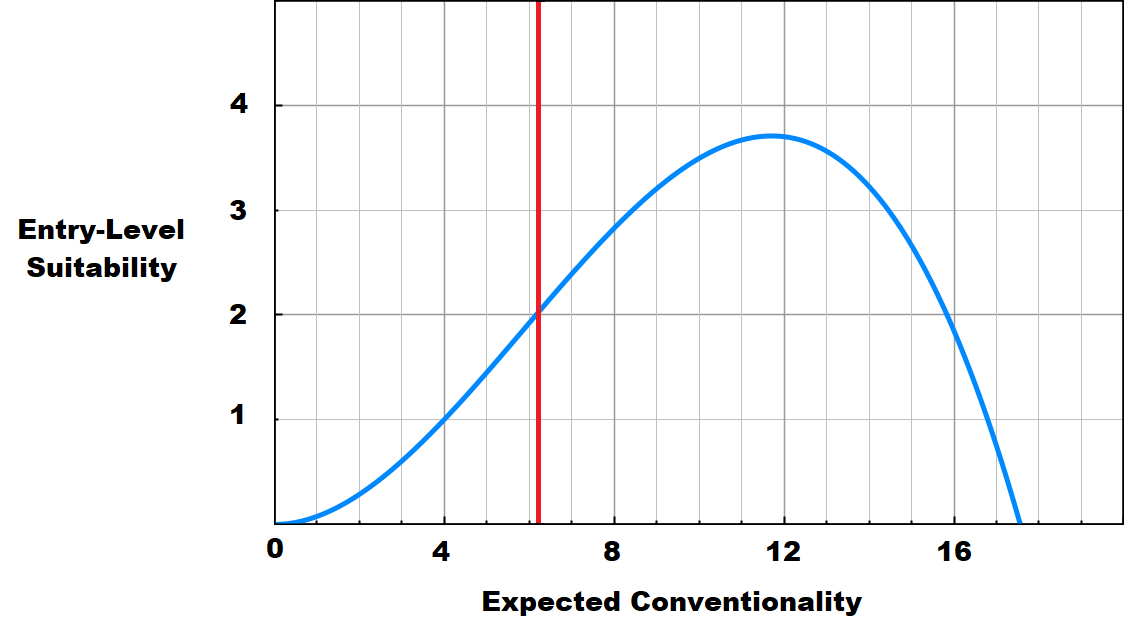
\includegraphics[width=0.7\textwidth]{./figures-and-tables/figure-3.png}};
            \node (n2) [above=0.25cm] at ($(n1)!0.5!(n1) - (6.2, 0)$) {\textbf{Suitability}};
            \node (n3) [above=0.25cm] at ($(n1)!0.5!(n1) - (0, 4)$) {\textbf{Expected Conventionality}};
    
            \end{tikzpicture}
    
        \label{fig:var_results}
        \end{figure}

    Figure \ref{fig:var_results} is a graphical representation of the VAR model results.
    Each model is a three-variable model with an H-1B impulse generating a first-order enrollment response,
    and both models leverage 23 observations over the period from 1994 to 2016.
    The loan model is optimized for four lags, with unanimous selection criteria assent.
    The CPI-adjusted tuition model presents mixed lag results.
    As previously discussed, I prefer the Schwarz Information Criterion because these models involve small sample sizes.
    SBIC indicates 3 lags as the optimal period for the CPI-adjusted tuition model.
    

    % TODO: var results summary paragraph

    \section{Conclusions}

    % the total effect of assistance in the relevant range is positive, and additional real assistance would further boost attendance.
    % however, it's not obvious that increased attendance is a good thing. credential inflation, experience inflation, debt crisis.
    % i fail to find evidence supporting a significant interaction between section 127 and visa policy
    % however visa policy in itself is extremely important in the conversation on enrollment, credential inflation, experience inflation, and debt crisis.
    % there are important caveats in this visa analysis.
    % employers have recently been removing the degree requirement
    % the law should also remove that requirement and boost alternative education which doesn't require a formal degree and is highly effective
    % this will reduce debt, improve diversity and economic efficiency and individual skill

    % maybe talk about stress and debt for why debt is important
    % important to look at wages not income (which would include investments, etc, see shrm's discussion: http://www.cpepea.com/wp-content/uploads/2017/05/10-0418-Coalition-Report-on-Public-Policy-Issue-E-P-E-A_FNL.pdf)
    % SHRM assessed only a single year, 2008. Shows Section 127 is mostly a Master's degree tool rn.
    % 75 percentile for salaries in 2017 was 54250 https://bizfluent.com/info-10032733-percentile-salary.html
    % define middle class as 50-75 percentile, lower class as under 50 percentile. break down effect by salary classification and see if it helps lower/middle
    % if so, it should improve diversity of education leading to a more diverse workforce which employers crave (TM) and politicians, etc...
    % Should we actually enact this policy? Effect on alternative credentials and credential inflation
    % Other options like extending the benefit to repayment https://blog.shrm.org/blog/let-s-fight-the-skills-gap-by-expanding-tax-free-education-assistance
    % we can also consider extending the education benefit to unaccredited education and income share agreements not just loans
    
    % https://www.nber.org/papers/w9225.pdf 
    % https://www.nber.org/digest/feb03/w9225.html

    \bibliography{./BibFile}
    
    \end{document}
        